\chapter{Robometer}
\label{sec:robometer}

This thesis builds directly on Robometer \citep{robometer}, so before turning to our own method we describe how it works in detail. In its own evaluation Robometer outperforms almost every prior vision-language reward model, which is why we build on it, the one exception being \citet{TRI-reward-model}, published a few weeks later. Our contributions change specific parts of this design, the data it learns from, the heads it trains, and the loss it minimizes, so the goal of this chapter is to introduce the baseline architecture and training objective to the reader. We cover the backbone it is built on and how it turns a video and an instruction into per-frame predictions, the three heads it carries and the objective that trains them, how those predictions serve as a reward, how progress and success are labeled, how clips become training samples, how it learns from comparisons, and the data it learns from. Figure~\ref{fig:robometer-overview} gives the model at a glance.

\begin{figure*}[t]
\centering
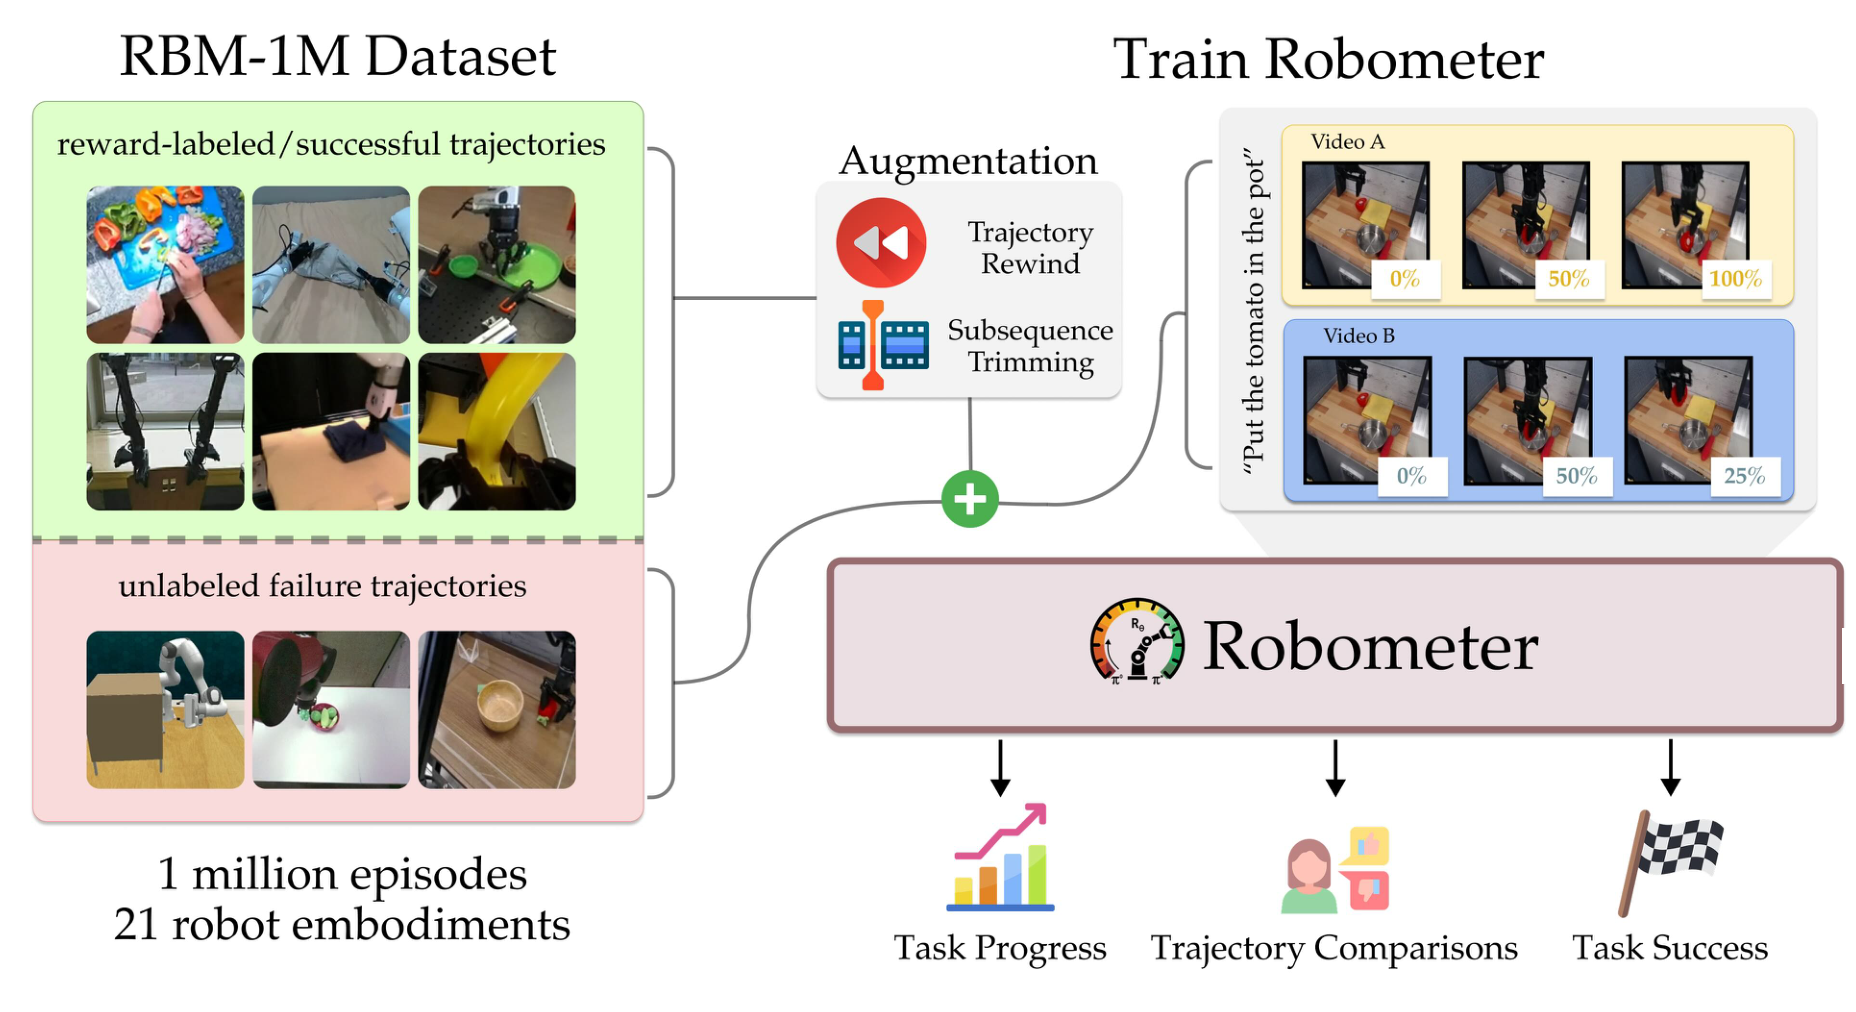
\includegraphics[width=0.85\textwidth]{media/robometer_overview.png}
\caption[Overview of Robometer]{An overview of Robometer, the reward model this thesis builds on, adapted from \citet{robometer}. Robometer is trained on RBM-1M, which pairs reward-labeled successful trajectories with unlabeled failures. During training these clips are augmented by trajectory rewind and subsequence trimming (Section~\ref{sec:bg-sampling}), and the model is supervised on three outputs, per-frame task progress, per-frame task success, and trajectory comparisons, which are the three heads this chapter describes.}
\label{fig:robometer-overview}
\end{figure*}

\section{Inputs and backbone}

Robometer is built on Qwen3-VL-4B-Instruct \citep{team_qwen3-vl_2025}, a pretrained vision-language model. Such a model has already learned, from large-scale image and text data, to recognize objects, read scenes, and connect them to language, and this prior knowledge is what lets a reward model generalize to tasks and robots it was not explicitly trained on. Robometer keeps this backbone and adapts it to scoring robot task videos.

A trajectory is presented as a short sequence of $T$ frames $o_1, \dots, o_T$ (with $T = 8$ in the paper's configuration) sampled evenly from the video, together with the task description $l$. To produce a prediction at each individual frame, Robometer inserts a learned progress token $\langle\mathrm{prog}\rangle$ directly after each frame. Writing $\mathrm{Tok}(\cdot)$ for the tokens an input produces, which for a video already carry the backbone's own video-start delimiter, the model sees
\begin{equation}
\mathrm{Tok}(l)\;\big[\,\mathrm{Tok}(o_t)\,\langle\mathrm{prog}\rangle\,\big]_{t=1}^{T} .
\label{eq:input-single}
\end{equation}
Robometer is also trained by comparison, learning which of two attempts at the same task is the better one, a preference-learning signal we return to in Section~\ref{sec:bg-comparisons}. This comparison uses a second input layout, in which two trajectories of the same task, $o^1$ and $o^2$, are placed one after the other, separated by a split token, with a single preference token $\langle\mathrm{pref}\rangle$ appended at the very end,
\begin{multline}
\mathrm{Tok}(l)\;\big[\,\mathrm{Tok}(o^1_t)\,\langle\mathrm{prog}\rangle\,\big]_{t=1}^{T}\;\langle\mathrm{split}\rangle\\
\big[\,\mathrm{Tok}(o^2_t)\,\big]_{t=1}^{T}\;\langle\mathrm{pref}\rangle .
\label{eq:input-pair}
\end{multline}
The state at this final preference token is what the model reads to decide which of the two trajectories, the first or the second, is the better attempt.

The backbone is causally masked, and this is what lets the model read every per-frame prediction from a single forward pass. In the single-trajectory input of Equation~\ref{eq:input-single}, the hidden state at the $t$-th progress token, which we write $h_t$, is the vector the backbone's final transformer layer outputs at that token's position, a single embedding of the model's hidden dimension. Because of the causal mask it can attend only to the instruction and to frames $1$ through $t$, so it is a running summary of the trajectory up to frame $t$. In the paired input of Equation~\ref{eq:input-pair}, the preference token sits after both trajectories and attends to all of them. The hidden states at these tokens, and nothing else, are what the prediction heads read.

\section{Three prediction heads}

Robometer attaches three lightweight heads on top of the shared backbone, each answering a different question.

\begin{itemize}
    \item \textbf{Progress.} For every frame, how far the task has advanced, on a scale from zero, meaning nothing has been accomplished, to one, meaning the task is complete. This is the dense, per-step signal that a policy can follow.
    \item \textbf{Success.} For every frame, whether the task has actually been completed, expressed as a probability. This is a standard binary reward that answers yes or no, instead of describing the percentage of the task that is complete.
    \item \textbf{Trajectory comparison.} Given two trajectories for the same task, which of the two is better. This head does not score a single trajectory in isolation. It orders a pair.
\end{itemize}

Each head is a small two-layer MLP applied to a progress or preference token's hidden state, and the three are trained together under a single objective,
\begin{equation}
\mathcal{L} = \mathcal{L}_{\mathrm{prog}} + \mathcal{L}_{\mathrm{succ}} + \mathcal{L}_{\mathrm{pref}} ,
\label{eq:total-loss}
\end{equation}
one term per head. We describe each head together with the loss that trains it. The per-frame targets these losses compare against, $p_t$, $s_t$, and $y$, are defined later in the chapter.

The \emph{success} head maps each progress-token state $h_t$ to a single logit, $\hat{s}_t = \sigma(\mathrm{MLP}_{\mathrm{succ}}(h_t)) \in [0,1]$, the probability that the task is complete at frame $t$. It is trained with a class-balanced binary cross-entropy against the binary target $s_t$,
\begin{equation}
\mathcal{L}_{\mathrm{succ}} = \frac{1}{T}\sum_{t=1}^{T} \mathrm{BCE}\!\big(s_t,\, \hat{s}_t\big).
\end{equation}

The \emph{progress} head is where Robometer departs from a plain regressor. Instead of predicting a single number, $\mathrm{MLP}_{\mathrm{prog}}(h_t)$ produces $N = 10$ logits, one for each of a fixed set of progress values, or bins, spaced evenly across $[0,1]$, following the C51 distributional formulation \citep{bellemare2017c51}. A softmax turns these logits into a distribution $\hat{p}_t \in \Delta^{N}$ over the bins, and a scalar progress value is read back as its expectation $\sum_{i=1}^{N} \hat{p}_{t,i}\, c_i$, where $c_i$ is the value of bin $i$. Modeling progress as a distribution, not a point estimate makes the target smoother to fit and lets the model express uncertainty about how far along it is. The head is trained with a cross-entropy between this distribution and the target progress encoded onto the same bins,
\begin{equation}
\mathcal{L}_{\mathrm{prog}} = \frac{1}{T}\sum_{t=1}^{T} \mathrm{CE}\!\big(\mathrm{Proj}(p_t),\, \hat{p}_t\big).
\end{equation}
The projection operator $\mathrm{Proj}(p_t)$ encodes the continuous ground-truth progress $p_t \in [0,1]$ into a target distribution over the $N$ bins. For $N=10$ the bins sit at $0.0, 0.11, 0.22, \dots, 1.0$, and since a true progress value rarely lands exactly on one, $\mathrm{Proj}$ splits a total mass of $1$ between the two closest bins, weighted by proximity. 

Consider a ground-truth progress of $p_t = 0.27$. It falls between the third bin ($0.22$) and the fourth ($0.33$), and since it is closer to $0.22$, the lower bin takes the larger share of the mass ($57\%$) and the upper bin the rest ($43\%$), chosen so that the mean of the target distribution reconstructs $p_t = 0.27$ exactly.

The \emph{preference} head maps the single preference-token state to one logit, $\hat{y} = \sigma(\mathrm{MLP}_{\mathrm{pref}}(h_{\langle\mathrm{pref}\rangle}))$, the probability that the first trajectory is the better of the pair. It is trained with a binary cross-entropy against the label $y \in \{0,1\}$ that marks which trajectory is better,
\begin{equation}
\mathcal{L}_{\mathrm{pref}} = -\big[\, y\log\hat{y} + (1-y)\log(1-\hat{y}) \,\big].
\label{eq:pref-loss}
\end{equation}

The success and progress heads produce the reward for a single trajectory and are the only ones used at deployment. The preference head needs a pair of trajectories, so it cannot score a lone trajectory and plays no role once the model is deployed; it exists only to shape training, in the way we make precise in Section~\ref{sec:bg-comparisons}, which is also why we do not include it in our own model.

\section{Using Robometer as a reward}

At deployment, Robometer takes a single trajectory and its task description and runs one forward pass. For each frame $t$ it reads the progress-token hidden state $h_t$ and passes it through the two task heads, which produce one success logit and $N = 10$ progress logits. A sigmoid on the success logit gives the per-frame success probability $\hat{s}_t$, and a softmax over the progress logits gives the per-frame progress distribution $\hat{p}_t$, whose mean is the scalar progress. The output of the model is therefore, for every frame, a success probability and a progress value.

A downstream reinforcement learning algorithm calls the model in place of a hand-designed or simulator reward and uses one of these per-frame quantities, the progress value or the success probability, as the reward signal. Because each frame's prediction depends only on the frames before it, the model can score a trajectory online as it grows, returning a reward at every step and not only at the end, which is what makes it usable inside a reinforcement learning loop.

The targets these heads are trained against, $p_t$ and $s_t$ for the two task heads and $y$ for the preference head, are where Robometer's design becomes consequential for our work, and we turn to how they are built next.

\section{How progress and success are labeled}

The progress head needs a dense per-frame target, and the success head a per-frame binary flag. Robometer obtains both cheaply for successful demonstrations by assuming that an expert demonstration advances steadily toward the goal. A demonstration of length $T$ is labeled by setting the progress target $p_t = t/T$, so it rises evenly from zero at the first frame to one at the last, while the success target $s_t$ is a binary flag, zero until the task is finished and one from completion onward. A frame one second into a two-second task is therefore marked half done. No human annotation is needed, because a successful demonstration reaches the goal by construction. There is one practical detail to note. A recording often keeps rolling for a moment after the task is already finished, so its final frames show no real progress. Robometer handles this by marking progress as complete slightly before the last frame, at a cutoff point chosen separately for each dataset.

As a concrete example, take a clip of a robot placing a cup on a shelf (Figure~\ref{fig:cup-labels}). The progress target climbs from zero as the arm reaches and lifts the cup, passes roughly one half as it carries the cup across, and reaches one as the cup settles on the shelf. The success target, by contrast, stays at zero for the entire approach and flips to one only at the moment the cup is in place.

\begin{figure*}[h]
\centering
% MetaWorld shelf-place success inst0000, eight of sixteen keyframes; progress = t/T.
\begin{tikzpicture}
\begin{axis}[scale only axis, width=0.944\textwidth, height=2.6cm,
  xmin=0.5, xmax=8.5, xtick=\empty, ymin=0, ymax=1.15, ytick={0,0.5,1},
  ylabel={Target}, axis lines=left, ymajorgrids, grid style={gray!18},
  tick label style={font=\scriptsize}, label style={font=\footnotesize},
  legend style={font=\scriptsize, at={(0.015,0.74)}, anchor=north west, draw=none, fill=none},
  legend cell align=left, enlarge x limits=false, clip=false]
\addplot[thick, mark=*, mark size=1.5pt, color=blue!65!black]
  coordinates {(1,0)(2,0.13)(3,0.27)(4,0.4)(5,0.6)(6,0.73)(7,0.87)(8,1)};
\addlegendentry{progress $p_t = t/T$}
\addplot[thick, dashed, color=orange!88!black]
  coordinates {(1,0)(6.5,0)(6.5,1)(8,1)};
\addlegendentry{success $s_t$}
\node[anchor=south, inner sep=0, yshift=2pt] at (axis cs:1,1.15) {
\includegraphics[width=0.118\textwidth]{media/sim/shelf_success/f0.jpg}};
\node[anchor=south, inner sep=0, yshift=2pt] at (axis cs:2,1.15) {
\includegraphics[width=0.118\textwidth]{media/sim/shelf_success/f1.jpg}};
\node[anchor=south, inner sep=0, yshift=2pt] at (axis cs:3,1.15) {
\includegraphics[width=0.118\textwidth]{media/sim/shelf_success/f2.jpg}};
\node[anchor=south, inner sep=0, yshift=2pt] at (axis cs:4,1.15) {
\includegraphics[width=0.118\textwidth]{media/sim/shelf_success/f3.jpg}};
\node[anchor=south, inner sep=0, yshift=2pt] at (axis cs:5,1.15) {
\includegraphics[width=0.118\textwidth]{media/sim/shelf_success/f4.jpg}};
\node[anchor=south, inner sep=0, yshift=2pt] at (axis cs:6,1.15) {
\includegraphics[width=0.118\textwidth]{media/sim/shelf_success/f5.jpg}};
\node[anchor=south, inner sep=0, yshift=2pt] at (axis cs:7,1.15) {
\includegraphics[width=0.118\textwidth]{media/sim/shelf_success/f6.jpg}};
\node[anchor=south, inner sep=0, yshift=2pt] at (axis cs:8,1.15) {
\includegraphics[width=0.118\textwidth]{media/sim/shelf_success/f7.jpg}};
\end{axis}
\end{tikzpicture}
\caption[Progress and success targets on a success clip]{The two training targets on a successful clip, a MetaWorld shelf-place episode that stands in for the cup example. Eight of sixteen keyframes are shown. Beneath them the progress target rises linearly with $t/T$ as the arm reaches, grasps, lifts, and places the block, while the success target stays at zero until the block is on the shelf and then jumps to one. A successful demonstration is labeled this way for free, with no annotation.}
\label{fig:cup-labels}
\end{figure*}

The same assumption fails for failures. A failed attempt does not advance evenly toward completion. It may stall at the start, move in the wrong direction, or come close to success and then fall apart, so a label like $t/T$ no longer reflects what is actually happening. Producing trustworthy per-frame progress labels for failures is therefore genuinely difficult, and Robometer sidesteps the difficulty by not labeling failures densely at all. This single decision is the starting point for our own work.

\section{From clips to training samples}
\label{sec:bg-sampling}

One more piece of Robometer's training recipe matters for what follows. The model is not trained on whole clips. Each training sample is a window cut from a stored trajectory, with boundaries drawn at random, and the frames inside the window receive fresh targets when the sample is built. On top of this windowing, Robometer generates progress samples through four strategies, drawn with equal probability. A \emph{forward} sample plays a window in its natural order, so its targets rise. A \emph{reverse} sample traverses the window backward, so its targets fall, teaching the model that progress can be undone. A \emph{rewind} sample runs forward and then back again, placing a regression in the middle of an otherwise normal clip; the authors ablate this strategy and find that removing it hurts failure detection. A \emph{different-task} sample keeps the frames but swaps in the instruction of another task and sets every progress target to zero, grounding the score in the instruction and not in motion alone. Our fine-tunes in Chapter~\ref{sec:methodology} inherit this sampling machinery unchanged, and it applies to our dense failure labels exactly as it does to the $t/T$ ramps, with the window's labels drawn from the stored per-frame values.

A second detail sits inside the same machinery. The success target is not labeled independently of progress. It is derived from it, with a frame marked complete exactly when its progress target reaches the completion cutoff described above. The two heads therefore share one labeling pipeline, and anything that shapes the progress targets shapes the success targets with it.

\section{Learning from comparisons}
\label{sec:bg-comparisons}

We now return to the third head, the preference head, and to the loss $\mathcal{L}_{\mathrm{pref}}$ of Equation~\ref{eq:pref-loss} that trains it. This head is what lets Robometer still benefit from the large pool of non-expert and failed trajectories, even without dense labels for them, and it does so through comparison, in the spirit of preference-based reward learning \citep{wang_rl-vlm-f_2024}. Given two trajectories of the same task, it sets the preference label $y = 1$ when the first is the better of the two and $y = 0$ otherwise, and trains the head to predict it through $\mathcal{L}_{\mathrm{pref}}$. A comparison needs only the relative ordering of the pair, not an exact value for either side, so it scales naturally to unlabeled and failed data, where a failed attempt simply becomes the lower-ranked side against an expert success.

The authors further report that comparisons help even when both trajectories succeed. Ranking a complete demonstration above a suboptimal but still successful one, for instance, gives the model an ordering signal that sharpens the progress and success heads without any failure data at all.

The consequence matters for this thesis. The progress and success heads learn almost entirely from successful trajectories, where the $t/T$ labels exist. Failed attempts reach the model only indirectly, as the lower-ranked side of a comparison. In other words, the two heads that actually generate the reward at deployment never see failure as a direct training target.

\section{Training data}

Robometer is trained on a corpus the authors call RBM-1M, roughly one million trajectories spanning twenty-one robot embodiments. It is drawn from public robot datasets, human videos, and simulation. Expert robot demonstrations form the largest single part, but a substantial share of the corpus comes from human video and from humanoid-robot data, which pushes its visual and embodiment coverage well beyond standard manipulator arms. We give a fuller breakdown of this corpus in Appendix~\ref{apx:rbm1m}, and of the changes we make to it in Appendix~\ref{apx:roboref-data}.
